\documentclass[a4paper,12pt]{article}
\usepackage[utf8]{inputenc}
\usepackage{polski}
\usepackage{graphicx}
\usepackage[lmargin=2cm,rmargin=2cm]{geometry}
\title{Najdłuższy cykl prosty w grafie}
\author{Kamil Chlebek, Arkadiusz Błasiak, Piotr Jaromin}
\begin{document}
\maketitle
\newpage
\tableofcontents
\newpage
\section{Teoria}
\subsection{Graf}

\textbf{Graf} to zbiór wierzchołków, które mogą być połączone krawędziami w taki sposób, że każda krawędź kończy się i zaczyna w którymś z wierzchołków

\begin{figure}[htbp]
\center{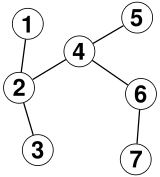
\includegraphics[scale=0.8]{grafnieskierowany.png}}
\caption{Graf nieskierowany}
\end{figure}
\subsection{Cykl}
\textbf{Cykl} jest ścieżką, która rozpoczyna się i kończy w tym samym wierzchołku (ścieżka ta może posiadać wielokrotnie ten sam wierzchołek). Cykl o długości 1 nazywa się pętlą.
\\
\\
\textbf{Cykl prosty} - jest ścieżką, która rozpoczyna się i kończy w tym samym wierzchołku (ścieżka ta nie może posiadać wielokrotnie tego samego wierzchołka)
\begin{figure}[htbp]
\center{
\includegraphics[scale=0.078]{hamilton.png}}
\caption{Cykl prosty w grafie}
\end{figure}
\subsection{Algorytm genetyczny}
\textbf{Algorytm genetyczny} - rodzaj algorytmu przeszukującego przestrzeń alternatywnych rozwiązań problemu w celu wyszukania rozwiązań najlepszych.
\subsubsection{Etapy algorytmu}
\begin{enumerate}
\item Losowanie początkowej populacji
\item Selekcja - populacja jest poddawana ocenie (korzystając z funkcji oceny), wybierane są najlepsze osobniki
\item Krzyżowanie - złączanie uprzednio wybranych osobników
\item Mutacja - wprowadzenie losowych zmian w osobniku
\item Rodzi się kolejne pokolenie. Najlepsze osobniki są powielane, a najsłabsze usuwane. Jeżeli nie przekroczono ilości iteracji, algorytm powraca do kroku drugiego. W przeciwnym wypadku wybieramy najlepszego osobnika z populacji.
\end{enumerate}
\subsubsection{Funkcja oceny}
Funkcja oceny to miara jakości dowolnego osobnika w populacji. Dla każdego osobnika jest ona ilością wierzchołków w ścieżce.
\subsubsection{Selekcja}
Za pomocą selekcji turniejowej wybieramy 2 osobniki, które poddajemy krzyżowaniu.
\subsubsection{Krzyżowanie}
Krzyżowanie zachodzi z pewnym prawdopodobieństwem(określonym przez użytkownika).
\\
Pierwsza połowa chromosomów z jednego osobnika jest łączona z drugą połową drugiego osobnika oraz druga połowa pierwszego z pierwszą połową drugiego. Wynikiem są dwa nowe osobniki. 
\begin{figure}[htbp]
\center{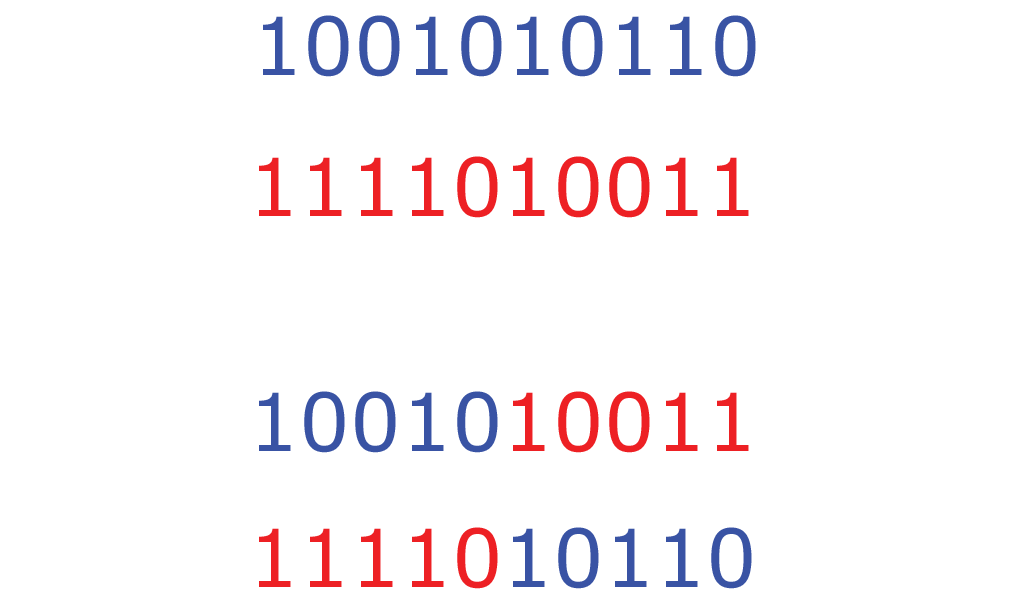
\includegraphics[scale=0.20]{krzyz.png}}
\caption{Krzyżowanie}
\end{figure}
\subsubsection{Mutacja}
Mutacja zachodzi z pewnym prawdopodobieństwem, które użytkownik może ustawić przed uruchomieniem programu (domyślnie wynosi 0.5). W wylosowanym miejscu w ścieżce dodajemy losowy wierzchołek przez który jeszcze nie przechodziliśmy. Proces jest powtarzany, aż do osiągnięcia prawidłowej ścieżki, bądź przekroczenia maksymalnej liczby iteracji
\begin{figure}[htbp]
\center{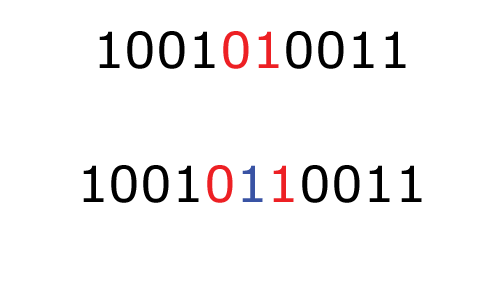
\includegraphics[scale=0.40]{mut.png}}
\caption{Mutacja}
\end{figure}
\section{Program}
\subsection{GUI}
\begin{figure}[htbp]
\center{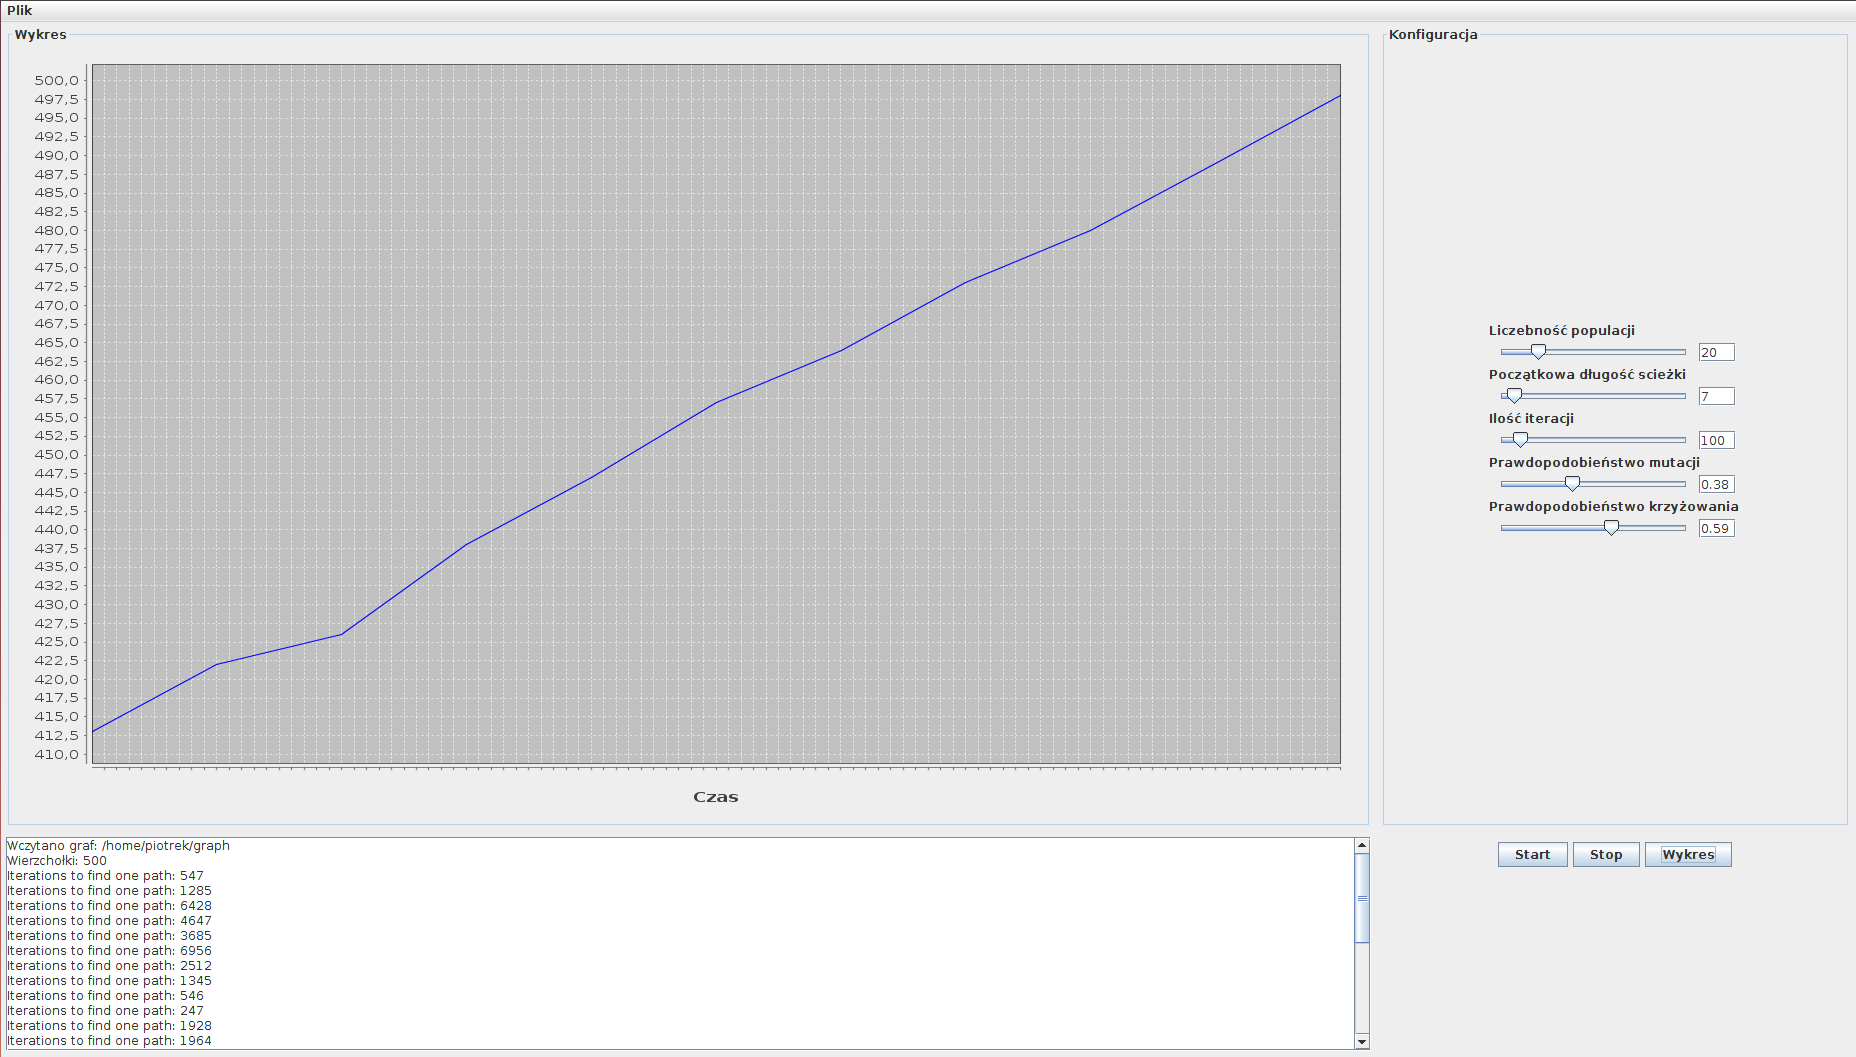
\includegraphics[scale=0.25]{interfejs.png}}
\caption{Interfejs programu}
\end{figure}
\subsubsection{Opis obszarów okna}
\begin{itemize}
\item \textbf{pole Wykres}: obrazuje zmianę populacji w zależności od czasu, jest generowany w czasie rzeczywistym
\item \textbf{pole Konfiguracja}: służy do ustalenia parametrów początkowych:
\begin{itemize}
\item \textbf{Liczebność populacji}: liczba naturalna z przedziału 1 - 100, określa ilość początkowych osobników
\item \textbf{Maksymalna początkowa długość ścieżki}: liczba naturalna z przedziału 2 - 100, określa przez maksymalnie ile wierzchołków przechodzi osobnik
\item \textbf{Prawdopodobieństwo mutacji}: ułamek z przedziału 0.0 - 1.0, określa prawdopodobieństwo zajścia mutacji
\item \textbf{Prawdopodobieństwo krzyżowania}: ułamek z przedziału 0.0 - 1.0, określa prawdopodobieństwo zajścia krzyżowania
\end{itemize}
\item \textbf{Obszar Logów}: wyświetla informacje dotyczące algorytmu
\item \textbf{Przycisk Start}: uruchamia program
\item \textbf{Przycisk Stop}: zatrzymuje program
\item \textbf{Przycisk Wykres}: pokazuje cały wykres
\end{itemize}
\subsection{Obsługa}
\subsubsection{Generowanie grafu}
\begin{figure}[htbp]
\center{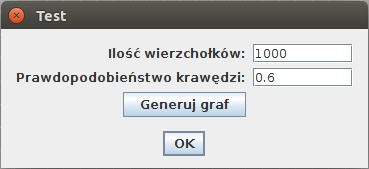
\includegraphics[scale=1]{generuj.png}}
\caption{Okno generowania grafu}
\end{figure}
\begin{enumerate}
\item Kliknij w przycisk "plik" znajdujący się w lewym górnym rogu programu;
\item Wybierz "Generuj graf";
\item W nowo otwartym oknie określ ilość wierzchołków i prawdopodobieństwo krawędzi;
\item Po kliknięciu "Generuj graf", wybierz ścieżkę do zapisania nowo utworzonego grafu.
\end{enumerate}
\newpage
\subsubsection{Wczytywanie grafu z pliku}
\begin{figure}[htbp]
\center{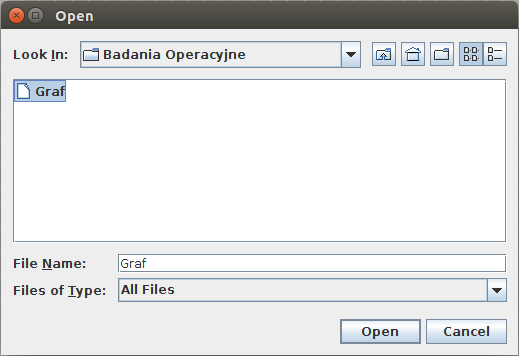
\includegraphics[scale=0.8]{open.png}}
\caption{Okno wczytywania grafu}
\end{figure}
\begin{enumerate}
\item Kliknij w przycisk "plik" znajdujący się w lewym górnym rogu programu;
\item Wybierz "Wczytaj graf";
\item Określ ścieżkę z zapisanym grafem;
\item Po kliknięciu "Open", program załaduje podany graf.
\end{enumerate}
\subsubsection{Znajdowanie najdłuższej ścieżki w grafie}
Po wczytaniu grafu kliknąć przycisk "start"
\end{document}